% Copyright 2005-2016 Airbus-EDF-IMACS-Phimeca
% Permission is granted to copy, distribute and/or modify this document
% under the terms of the GNU Free Documentation License, Version 1.2
% or any later version published by the Free Software Foundation;
% with no Invariant Sections, no Front-Cover Texts, and no Back-Cover
% Texts.  A copy of the license is included in the section entitled "GNU
% Free Documentation License".
\renewcommand{\nomfichier}{docref_C311_Sorm}
\renewcommand{\titrefiche}{SORM}

\Header

\MathematicalDescription{

  \underline{\textbf{Goal}} \vspace{2mm}

  The Second Order Reliability Method is used in the same context as the First Order Reliability: refer to \otref{docref_C311_Form}{FORM} for further details.
  The objective of SORM is to evaluate the probability content of the event $\cD_f = \{\vect{X} \in \Rset^n \, / \, g(\vect{X}\,,\,\vect{d}) \le 0\}$ :
  \begin{equation}\label{PfX4}
    P_f = \Prob{g(\vect{X}\,,\,\vect{d})\leq 0}=   \int_{\cD_f}  \pdf\, d\vect{x}
  \end{equation}

  \vspace{2mm}

  \underline{\textbf{Principle}}

  \begin{center}
    % 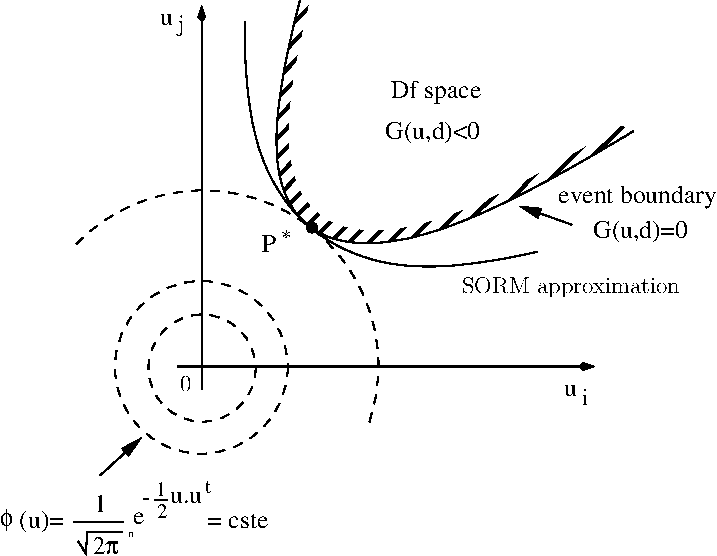
\includegraphics[scale=0.8]{Figures/FigureSorm.pdf}
  \end{center}

  The principle is the same as for FORM. After having mapped the physical space into the standard through an isoprobabilistic transformation (refer to  \otref{docref_C311_TransIso}{Isoprobabilistic Transformation}), eq. (\ref{PfX4}) becomes :
  \begin{equation}\label{PfU2}
    P_f = \Prob{G(\vect{U}\,,\,\vect{d})\leq 0} = \int_{\Rset^n} \boldsymbol{1}_{G(\vect{u}\,,\,\vect{d}) \leq 0}\,f_{\vect{U}}(\vect{u})\,d\vect{u}
  \end{equation}
  where $f_{\vect{U}}$ is the density function of the distribution in the standard space :  that distribution is spherical (invariant by rotation by definition). That property implies that $f_{\vect{U}}$ is a function of $||\vect{U}||^2$ only. Furthermore, we suppose that outside the sphere which tangents the limit state surface in the standard space, $f_{\vect{U}}$ is decreasing. \\
  The difference with FORM comes from the approximation of the limit state surface at the design point $ \vect{P}^*$ in the standard space : SORM approximates it by a quadratic surface that has the same main curvatures at the design point.\\

  Let us denote by $n$ the dimension of the random vector $\vect{X}$ and $(\kappa_i)_{1 \leq i \leq n-1}$ the $n-1$ main curvatures of the limit state function at the design point in the standard space.\\

  Several approximations are available in the standard version of OpenTURNS, detailed here in the case where the origin of the standard space does not belong to the failure domain : \\

  \begin{itemize}
  \item Breitung's formula is an asymptotic results (see [Breitung]: the usual formula used in the normal standard space, has been generalized in [R. Lebrun, A. Dutfoy, 2008, b] to standard spaces where the distribution is spherical, with $E$ the marginal cumulative density function of the spherical distributions in the standard space (see  \otref{docref_C311_TransIso_Generalized Nataf}{Generalized Nataf}) :
  \end{itemize}
  \begin{equation}
    \label{PfSORM_B}
    P_{Breitung}^{generalized}  \stackrel{\beta\rightarrow\infty}{=} E(-\beta)\prod_{i=1}^{n-1}\frac{1}{\sqrt{1+\beta\kappa_i}}
  \end{equation}
  where $\Phi$ is the cumulative distribution function of the standard 1D normal distribution.

  \begin{itemize}
  \item Hohenbichler's formula is an approximation of equation (\ref{PfSORM_B}):
    \begin{equation}
      \label{PfSORM_HB}
      \displaystyle P_{Hohenbichler} = \Phi(-\beta_{HL}) \prod_{i=1}^{n-1} \left( 1+\frac{\phi(-\beta_{HL})}{\Phi(-\beta_{HL})}\kappa_i  \right)  ^{-1/2}
    \end{equation}
        {\bf This formula is valid only in the normal standard space  and if $\boldsymbol{\forall i, 1+\frac{\phi(-\beta_{HL})}{\Phi(-\beta_{HL})}\kappa_i > 0}$}.
      \item Tvedt's formula (Tvedt, 1988) :
        \begin{equation}
          \label{PfSORM_T}
          \left\{
          \begin{array}{lcl}
            \displaystyle P_{Tvedt} & = & A_1 + A_2 + A_3 \\
            \displaystyle A_1 & = &  \displaystyle \Phi(-\beta_{HL}) \prod_{i=1}^{N-1} \left( 1+\beta_{HL} \kappa_i \right) ^{-1/2}\\
            \displaystyle A_2 & = &   \displaystyle\left[ \beta_{HL}  \Phi(-\beta_{HL}) -  \phi(\beta_{HL})\right ]  \left[  \prod_{j=1}^{N-1}  \left( 1+\beta_{HL} \kappa_i \right) ^{-1/2} -    \prod_{j=1}^{N-1}  \left( 1+(1 + \beta_{HL}) \kappa_i \right) ^{-1/2} \right ] \\
            \displaystyle A_3 & = &  \displaystyle(1 + \beta_{HL}) \left[ \beta_{HL}  \Phi(-\beta_{HL}) -  \phi(\beta_{HL})\right ]  \left[  \prod_{j=1}^{N-1}  \left( 1+\beta_{HL} \kappa_i \right) ^{-1/2} \right.\\
              & & \displaystyle\left. - {\cR}e \left(   \prod_{j=1}^{N-1}  \left( 1+(i + \beta_{HL}) \kappa_j \right) ^{-1/2}  \right)\right ]
          \end{array}
          \right.
        \end{equation}
        where $ {\cR}e(z)$ is the real part of the complex number $z$ and $i$ the complex number such that $i^2 = -1$ and $\Phi$ the cumulative distribution function of the standard 1D normal distribution.\\
        {\bf This formula is valid only in the normal standard space  and if $\boldsymbol{\forall i, 1+\beta \kappa_i > 0}$ and $\boldsymbol{\forall i, 1+(1 + \beta) \kappa_i> 0}$}.
  \end{itemize}

}
{
  --}


\Methodology{
  Within the global methodology, the Second Order Reliability Method is used in the step C : "Uncertainty propagation" in the case of the evaluation of the probability of an event
  by an approximation method.\\
  It requires to have fulfilled the following steps beforehand:
  \begin{itemize}
  \item step A1: identify of an input vector $\vect{X}$ of sources of uncertainties and an output variable of interest $Z=\tilde{g}(\vect{X},\vect{d})$, result of the model $\tilde{g}()$; identify a probabilistic criteria such as a threshold exceedance $Z > z_s$ or equivalently a failure event ${g(\vect{X}\,,\,\vect{d}) \le 0}$,
  \item step B: identify one of the proposed techniques to estimate a probabilistic model of the input vector $\vect{X}$,
  \item step C: select an appropriate optimization algorithm among those proposed.
  \end{itemize}

  The Second Order Reliability Method provides the following results :
  \begin{itemize}
  \item the SORM probabilities calculated in Eqs. (\ref{PfSORM_B}),(\ref{PfSORM_HB}), (\ref{PfSORM_T})
  \item the importance factors associated to the event : refer to \otref{docref_Cprime31_FactImp}{Importance Factors} to obtain details,
  \item if asked by user, the sensitivity factors associated to the event : refer to \otref{docref_Cprime31_FactSens}{Sensitivity Factors} to obtain details.
  \end{itemize}
}
{
  The motivations for using SORM are similar to the motivations for using FORM. As it takes into account the curvatures of the limit state surface, SORM is usually more accurate than FORM e.g. in case when the event boundary is highly curved.\\

  The evaluation of the previous formulas requires that the limit state function be twice differentiable at the design point.\\

  The quality of the results obtained by the Second Order Reliability Method depends on the quality of the design point (same points as the FORM approximation), on the shape of the event boundary which must be well approximated by a quadratic surface near the design point and on the accuracy of the computed curvatures, which depends on the accuracy of both the evaluation of the gradient and the hessian at the design point.\\

  The Tvedt formula is exact for a quadratic surface and asymptotically exact for another types of surfaces. The Hohen-Bichler formula is a variant as regards to the Breitung one.\\

  At last, let us note that the SORM approximation depend on the geometry of the limit state function in the standard space and thus it depends on the isoprobabilistic transformation used. In the normal copula case, [R. Lebrun, A. Dutfoy, 2008, c] has showed that both isoprobabilistic transformations are identical and then the SORM approximations are identical too. But, in all the other cases, both isoprobabilistic transformations lead to different standard spaces and thus to different SORM approximations. As the same way, the conditioning order in the Rosenblatt transformation has also an impact on the SORM approximations when the copula of the random vector $\vect{X}$ is not normal.\\

  Let us note some useful references :
  \begin{itemize}
  \item Breitung K. a, "Asymptotic approximation for probability integral," Probability Engineering Mechanics, 1989, Vol 4, No. 4.
  \item Breitung K. b, 1984, "Asymptotic Approximation for multinormal Integrals," Journal of Engineering Mechanics, ASCE, 110(3), 357-366.
  \item Hohenbichler M., Rackwitz R., 1988, "Improvement of second order reliability estimates by importance sampling," Journal of Engineering Mechanics, ASCE,114(12), pp 2195-2199.
  \item R. Lebrun, A. Dutfoy, b, 2008, "A generalisation of the Nataf transformation to distributions with elliptical copula", Probabilistic Engineering Mechanics 24 (2009), pp. 172-178, doi:10.1016/j.probengmech.2008.05.001.
  \item R. Lebrun, A. Dutfoy, 2008, c, "Do Rosenblatt and Nataf isoprobabilistic transformations really differ?", submitted to Probabilistic  Engineering Mechanics in august 2008, under review so far.
  \item Tvedt L. 1988, "Second order reliability by an exact integral," proc. of the IFIP Working Conf. Reliability and Optimization of Structural Systems, Thoft-Christensen (Ed), pp377-384.
  \item Zhao Y. G., Ono T., 1999, "New approximations for SORM : part 1", Journal of Engineering Mechanics, ASCE,125(1), pp 79-85.
  \item Zhao Y. G., Ono T., 1999, "New approximations for SORM : part 2", Journal of Engineering Mechanics, ASCE,125(1), pp 86-93.
  \item Adhikari S., 2004, "Reliability analysis using parabolic failure surface approximation", Journal of Engineering Mechanics, ASCE,130(12), pp 1407-1427.
  \end{itemize}
}

\Example{

  Let's apply this method to the following analytical example which considers a cantilever beam, of Young's modulus E, length L, section modulus I. We apply a concentrated bending force at the other end of the beam. The vertical displacement $y$ of the extreme end is equal to :
  \begin{align*}
    y(E, F, L, I) = \displaystyle \frac{FL^3}{3EI}
  \end{align*}
  The objective is to propagate until $y$ the uncertainties of the variables $(E, F, L, I)$.\\
  The input random vector is $\vect{X} = (E, F, L, I)$, which probabilistic modelling is (unity is not provided):
  \begin{align*}
    \left\{
    \begin{array}{lcl}
      E & = & Normal(50, 1) \\
      F & = & Normal(1, 1) \\
      L & = & Normal(10, 1) \\
      I & = & Normal(5, 1)
    \end{array}
    \right.
  \end{align*}
  The four random variables are independent.\\

  The event considered is the threshold exceedance : $\cD_f = \{(E, F, L, I) \in \Rset^4 \, / \, y(E, F, L, I) \ge 3\}$
  We obtain the following results :
  \begin{align*}
    \left\{
    \begin{array}{lcl}
      P_{Breitung} & = & 2.5491 e^{-1}\, \% \\
      P_{Hohenbichler} & = & 2.648 e^{-1}\, \% \\
      P_{Tvedt} & = & 2.601e^{-1}
    \end{array}
    \right.
  \end{align*}
  These three approximations are coherent between them, which increases confidence in these results.
}
